\chapter{In-Context Learning}\label{chap:in-context-learning}

This chapter provides an overview of the in-context learning paradigm in relation to the thesis objectives. It begins with a definition, continues with a discussion of long context, and concludes with the relevance of in-context learning to the code completion task.

\section{Definition}

In-Context Learning (ICL) refers to the ability of a model to condition on a set of demonstrations provided in the input context in order to learn and adapt to unseen tasks without modifying its parameters \parencite{brown2020}. The input string is called a \textit{prompt}, and typically includes a task description along with a set of examples. The process of constructing a prompt to better leverage ICL is referred to as \textit{prompt engineering}.

This learning paradigm has proven highly effective, as it enables specialized approaches to solving tasks based solely on inference computations, while the model is pre-trained without awareness of task specificity.

\section{Long Context}

ICL introduces context length as a new scaling direction for LLMs \parencite{kaplan2020}, as shown in \figureref{fig:context-power-law}. The terminology also encompasses the concepts of \textit{zero-shot}, \textit{one-shot}, and \textit{few-shot prompting}, which refer to the number of demonstrations provided in the prompt. Increasing the number of demonstrations typically leads to improved downstream performance \parencite{brown2020}.

\begin{figure}[ht]
    \centering
    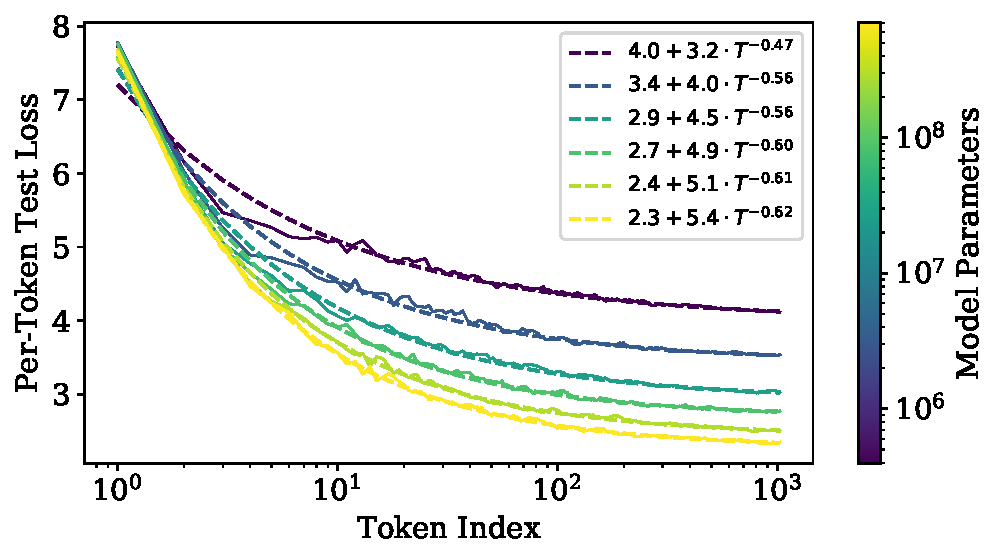
\includegraphics[width=\textwidth]{figures/context-power-law.pdf}
    \shortcaption{Power-law scaling of test loss with context token position}{Power-law scaling of test loss with context token position}\label{fig:context-power-law}
    \hfill\textit{Source: \citet{kaplan2020}}
\end{figure}

However, leveraging the advancements of this scaling direction requires addressing multiple challenges. The following overview develops a fundamental understanding of some of the directions associated with long context in the field.

\subsection{Quadratic Complexity of Attention}

The original attention architecture of Transformer models exhibits quadratic computational and time complexity requirements, which depend on the number of tokens provided to the model \parencite{vaswani2017}. This undesirable property has prompted the development of numerous subquadratic and other efficient attention mechanisms. For instance, the survey by \citet{tay2022} offers a detailed examination of this subject and visualizes the taxonomy of such architectures, as shown in \figureref{fig:taxonomy-of-transformers}.

\begin{figure}[ht]
    \centering
    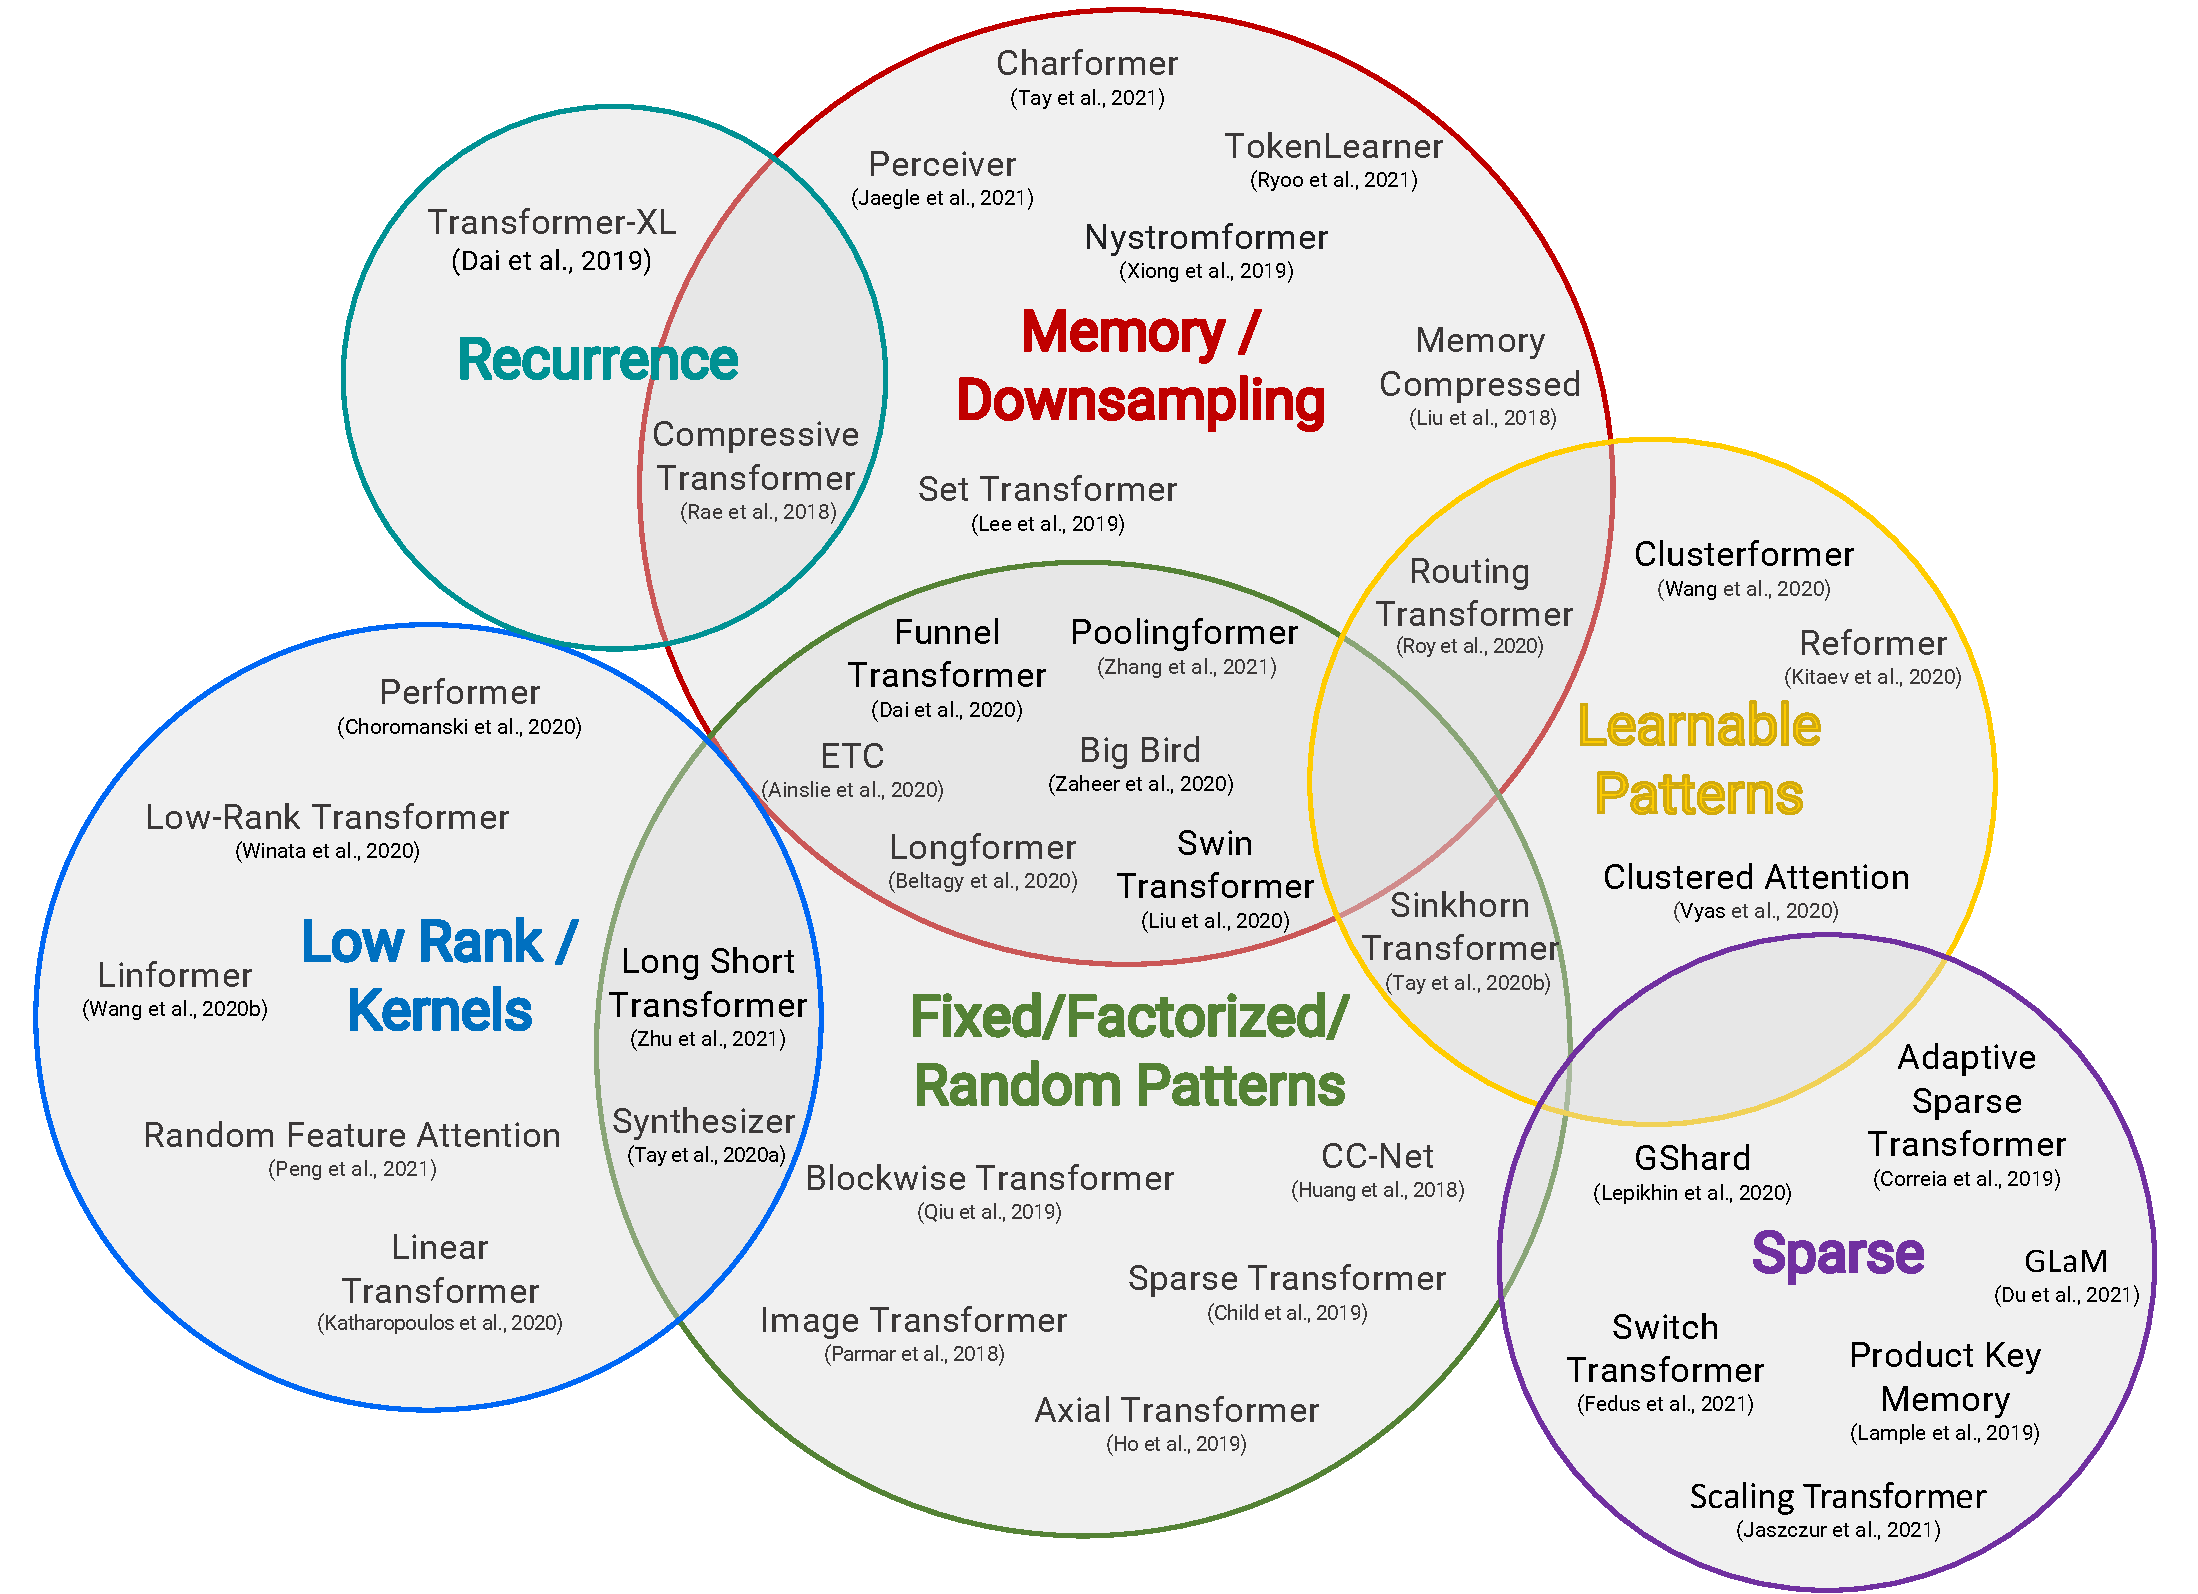
\includegraphics[width=\textwidth]{figures/taxonomy-of-transformers.pdf}
    \shortcaption{Taxonomy of efficient Transformer architectures}{Taxonomy of efficient Transformer architectures}\label{fig:taxonomy-of-transformers}
    \hfill\textit{Source: \citet{tay2022}}
\end{figure}

\subsection{Retrieval-Augmented Generation}

Not only the number of demonstrations but also their relevance to the task has been proven to be a crucial factor in ICL performance \parencite{liu2021}. Given a limited upper bound on the context length of the prompt, the task of finding the most relevant grounding information has become an important component of the respective research.

Closely related to this idea is the Retrieval-Augmented Generation (RAG) framework, which introduces a separate retrieval step in the prompt engineering procedure \parencite{lewis2020}. The objective of this mechanism is to provide the model with access to a non-parametric chunk of information related to the task at hand. The provided context can be either a factual knowledge supplement or the demonstrations required by the ICL setting.

\newpage
\begin{sloppypar}
RAG addresses the problem of overfitting and updates the outdated parameter-based memory of the model with a more relevant, query-conditioned context.
\end{sloppypar}

\subsection{Context Extension}

Since long context is an obstacle present at the architectural level, it affects both the inference and training modes of the model. The latter is particularly problematic, as it is more resource intensive. This issue is mitigated by dividing the model development pipeline into multiple stages, the specific cases for Code LLMs of which are discussed in \sectionref{sec:training-stages}. First, models are heavily trained on a small context window, which is then extended to larger ones. This approach drastically reduces training time and long context data requirements, thereby increasing the efficiency of the pipeline \parencite{xiong2023}.

\textit{Context extension} is functionally linked to RoPE, as the only novel information passed to the model with longer contexts is the greater positional span. This necessitates the introduction of an extrapolation property for this information. However, this cannot be directly achieved by simply training on longer sequences, as RoPE has been shown to be a universal approximator and suffers greatly on ranges outside of the original context window \mbox{\parencite{chen2023}}. To address this issue, multiple methods have been proposed (\cite{chen2023};~\cite{rozière2023};~\cite{peng2023};~\cite{xiong2023}), the main idea of which is to shift from the landscape of the extrapolation problem to that of interpolation.

The most fundamental modification in the model's architecture between short and long training stages is an Adjustment of the Base Frequency (ABF) parameter of RoPE, as concurrently proposed by \citet{rozière2023} and \citet{xiong2023}. More specifically, \(\theta_{\mathrm{base}}\) is scaled by one or two orders of magnitude to diminish the decay of the attention scores related to the increased relative distance \(m - n\) between tokens.

\section{Code Completion Prompting}

ICL emerges during the training of large language models via the next-token prediction objective as a function of the number of parameters and the data size used for pre-training \parencite{hahn2023}. Thus, its presence is found in base models, which are used to perform the code completion task.

In this thesis, individual demonstrations are not distinguished, and the prompt is treated as a set of concatenated text snippets, which consist of the content of repository text files and are organized according to RAG principles, where the completion file serves as a query.
